\documentclass[../../main]{subfiles}
\begin{document}

\subsection{Server implementation choices}
\label{ss:server-implementation-choices}

In \ref{ss:backend-architecture} we expressed how the backend is designed from a high-level perspective and how the different parts of it should communicate between each other.\\
We shall now present the choices we took in terms of technologies and implementation of the actual parts.

\begin{figure}[h]
    \centering
    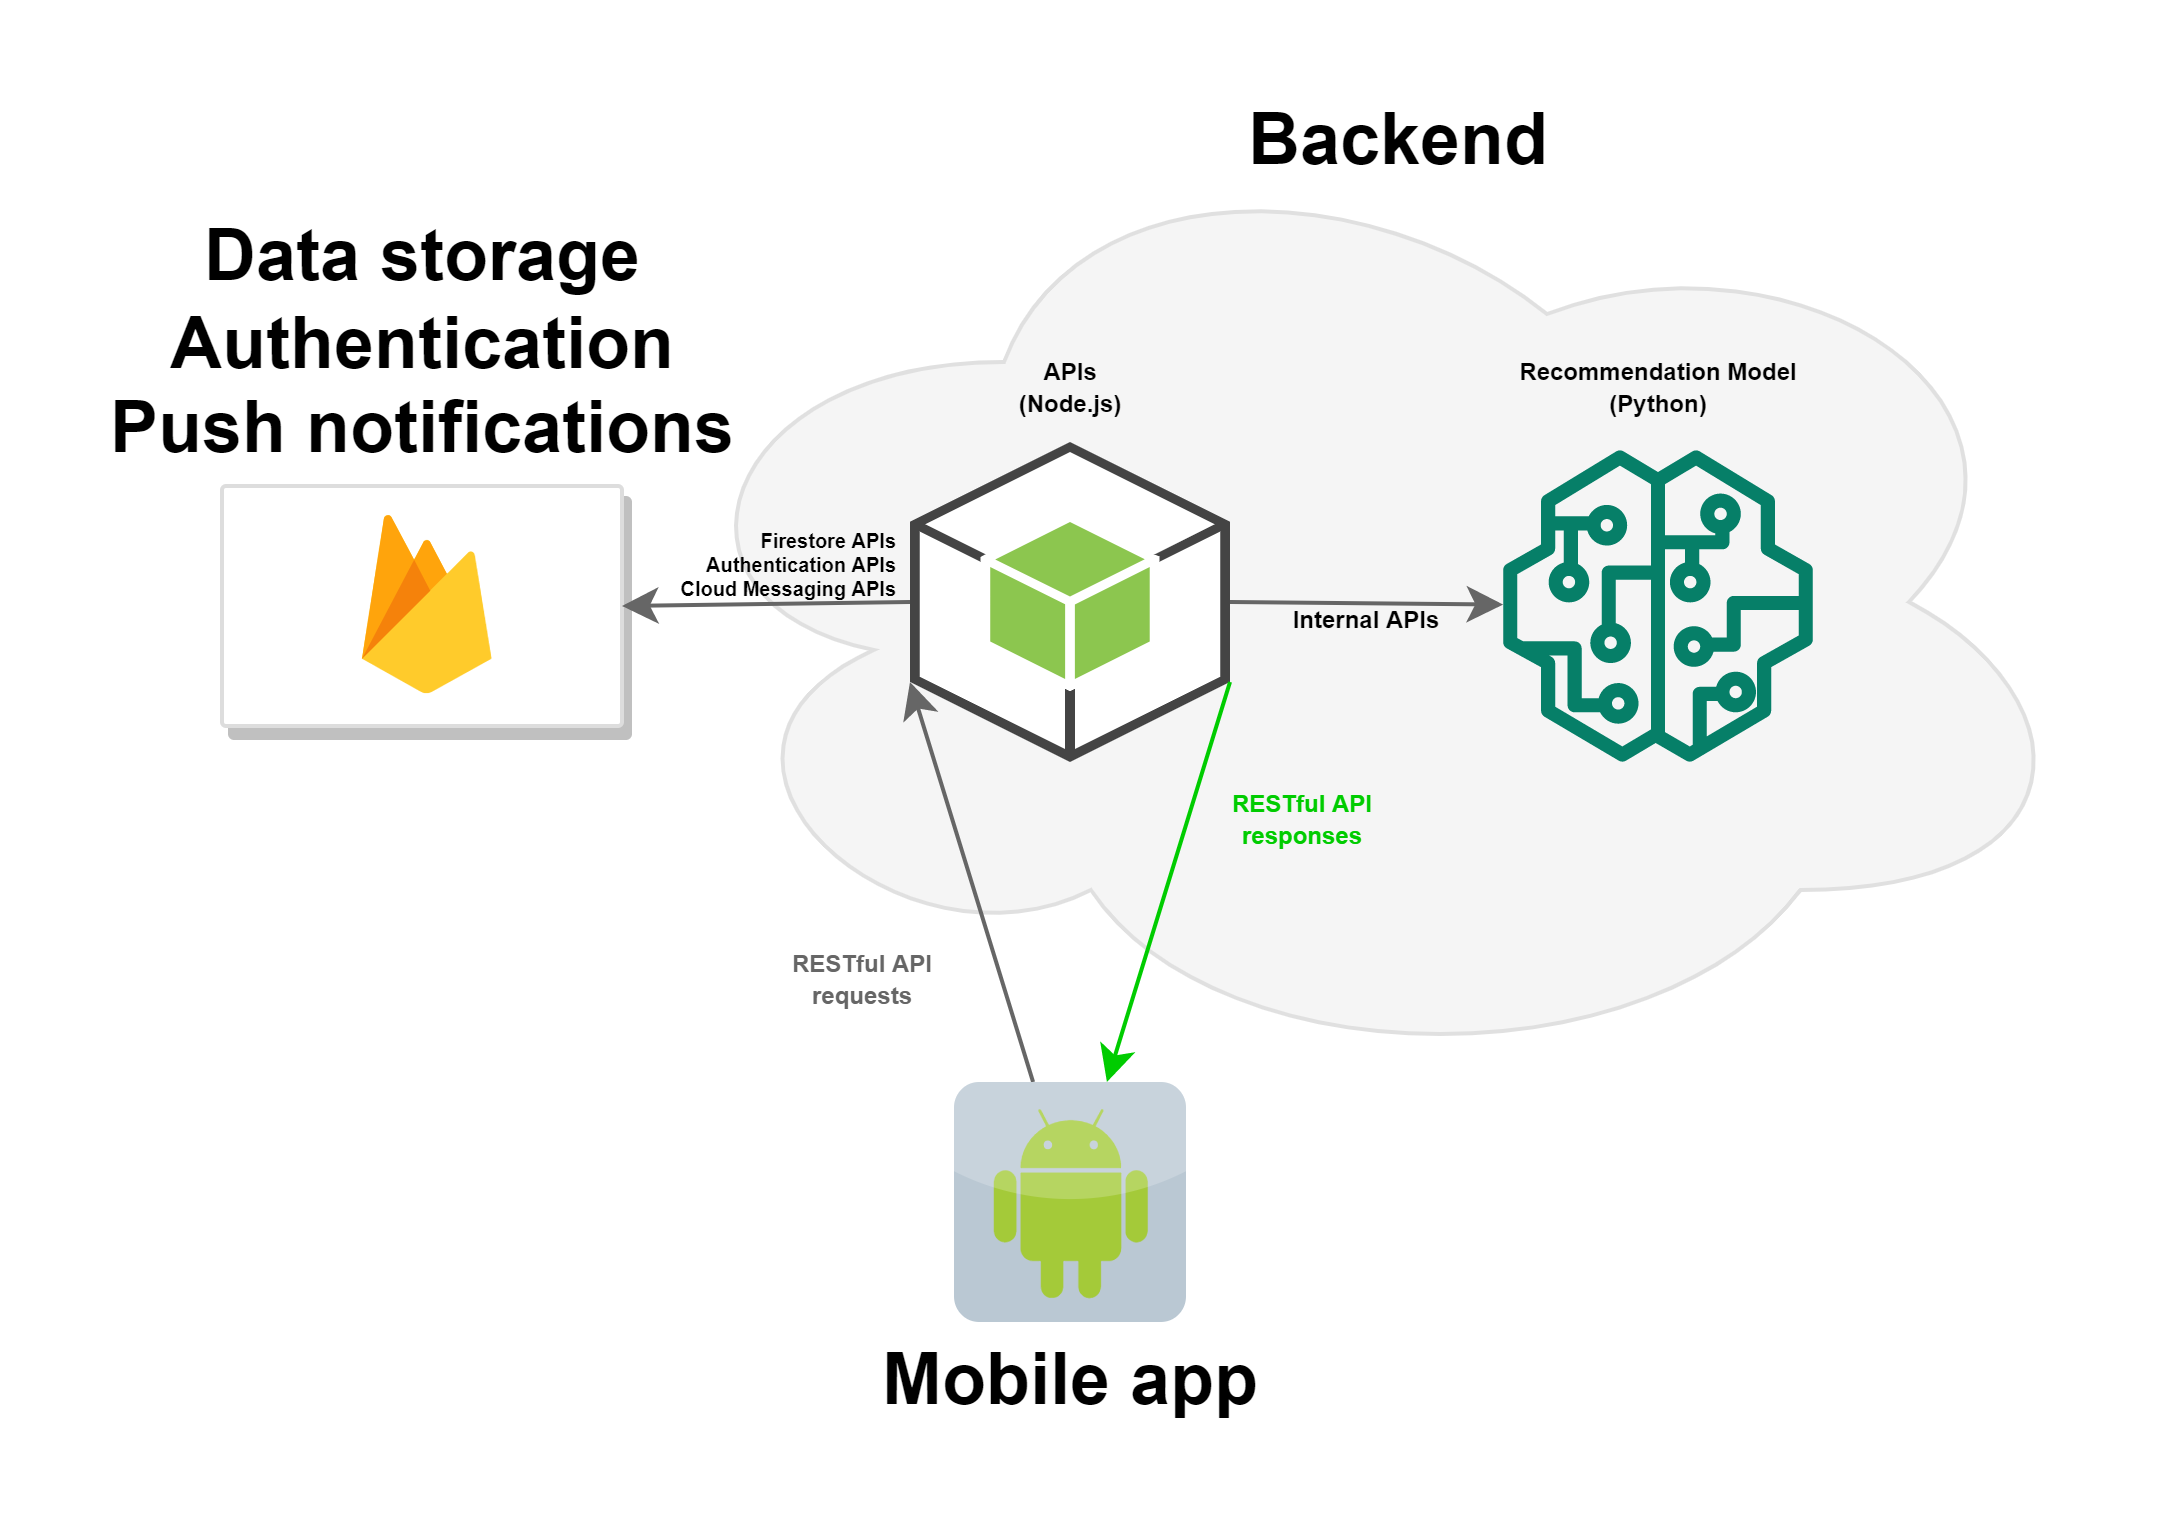
\includegraphics[width=0.8\textwidth]{images/backend_architecture_technologies}
    \caption{Backend architecture (in terms of technologies)}\label{fig:backend_architecture_technologies}
\end{figure}

\subsubsection{APIs}
\label{sss:apis}

The APIs of the backend are implemented mainly with \textbf{Node.js} and the library \textbf{Express}.
The choice of the former was made because of the ease of setup it required for getting started and for its ease of configuration compared to other frameworks;
the latter came naturally since it is the most widespread library for implementing RESTful APIs with Node.js.\\
The Node.js instance is used to handle the internal communications with:
\begin{itemize}
    \item the data storage, implemented with \textbf{Firestore}, accessed via the \textbf{Firebase Admin} library;
    \item the authentication service, implemented via \textbf{Firebase Authentication}, accessed via the \textbf{Firebase Admin} library;
    \item the push notifications service, implemented with \textbf{Firebase Cloud Messaging}, accessed via the \textbf{Firebase Admin} library;
    \item the recommendation model part of the backend, implemented with \textbf{Python}, accessed via the \textbf{Superagent} HTTP client library.
\end{itemize}
\noindent
Let's now see the methods available to use for the client:
\begin{enumerate}[I)]
    \item \texttt{/user-data}
    \begin{enumerate}[i)]
        \item \texttt{/notification-token} Sends the notification token for storing it (POST);
        \item \texttt{/public-key} Sends the user's device RSA public key for storing it (POST);
    \end{enumerate}

    \item \texttt{/points-of-interest}:
    \begin{enumerate}[i)]
        \item \texttt{/} Retrieves a user's \textit{pois} list (GET);
        \item \texttt{/add} Adds a \textit{poi} to those of the user (POST);
        \item \texttt{/remove} Removes a \textit{poi} from those of the user (DELETE);
    \end{enumerate}

    \item \texttt{/live-events}:
    \begin{enumerate}[i)]
        \item \texttt{/} Get the user's live events list (GET);
        \item \texttt{/add} Adds a live event to those of the user and their friends (POST);
    \end{enumerate}

    \item \texttt{/friends}:
    \begin{enumerate}[i)]
        \item \texttt{/} Get the user's friends list (only those that were confirmed) (GET);
        \item \texttt{/add} Sends a friendship request (POST);
        \item \texttt{/confirm} Confirms a friendship request (POST);
        \item \texttt{/deny} Denies a friendship request (POST);
        \item \texttt{/remove} Removes a friend (DELETE);
    \end{enumerate}
    
    \item \texttt{/recommendation}
    \begin{enumerate}[i)]
        \item \texttt{/places} Gets a place recommendation for whatever category (POST);
        \item \texttt{/validity} Gets a place recommendation only if the category makes sense with the input data (POST);
        \item \texttt{/train} Trains again the classifier inside the recommendation model with the additional user's feedback (POST).
    \end{enumerate}
\end{enumerate}

\subsubsection{Recommendation model}
\label{sss:recommendation-model-development}

The recommendation model of the backend is developed in Python and it is essentially composed by two parts:
\begin{itemize}
    \item the RESTful APIs exposed to the backend main APIs, implemented with the \textbf{Flask} library;
    \item the actual classifier, trained on the training dataset and the data coming from users, of which we talked about in \ref{sss:recommendation-model-design}, implemented with the \textbf{Scikit-learn} library.
\end{itemize}
% After the data synthetization we build the dataset used as input to train our model. First of all we separeted the place cateogry columns because it represent the results that we want to predict, and we removed some useless information from the dataset like the data returned from Places API, the outliers and the cluster index.
% \paragraph*{Oversample}
% We oversampled the dataset with two mechanism:
% \begin{itemize}
%     \item \textbf{RandomOverSampler} from imblearn;
%     \item \textbf{get\_dummies} from pandas.
% \end{itemize}

% We used RandomOverSampler to oversample X and y, and get\_dummies to oversample X relative to human activity
% because they are saved as string. We also one hot encoding the human activity to give more meaning to this value on the dataset.

% \paragraph*{Train}
% We used the 70\% of the dataset to perform the training and we used a \textbf{Decision Tree Classifier} to train a model able to
% predict the place category. 
% With a request input made of:
% \begin{itemize}
%     \item Seconds of day;
%     \item Day of week;
%     \item Latitude;
%     \item Longitude;
%     \item Human activity encoded.
% \end{itemize}
% As said in \namerefLabeled{paragraph:train_design} we thought that the recommendation model should follow a path like \textit{' At this \textbf{Hour} in this \textbf{Day} in this \textbf{position} by doing this \textbf{human activity} the best place is \textbf{place category}. '}.
% Talking about node of the tree. This is due the fact we want to discriminate determinate category by the time of the day and the human activity we are performing.
% Ideally a user goes to the gym during the week but probably in the evening or early morning, 
% goes to a restaurant/bar in any day at breakfast, launch or dinner time and he is probably walking or still on that place.
% But probably he goes to some leisure place during the weekend in the middle morning, afternoon or any day after dinner in the evening/night.

% The latitude and longitude is used to further discriminate some activity in any places because the data collected from the users could change due to their different attitude in the various part of the world.
% (Most of the point are from USA or China)
% \paragraph*{Test}
% After the train we tested the model obtained with the remaining 30\% of the oversampled dataset and we have instantly obtained and accuracy near to 65\%, that is very high due to the small dataset that we obtained from the preprocessing.
% Also we tried some recommendation request from the android client emulator and we received decent predictions. To continue improving the model we implemented the possibility to retrain it by adding the recommendation that the client has received, modified with the right category if he feels that the prediction didn't suit his needs. 

\subsubsection{Security}
\label{sss:security}

For the reasons expressed in \ref{ss:security-in-communication}, some security mechanism needed to be implemented for avoiding sensitive data of users being exposed or intercepted easily.
Those security mechanism are:
\begin{itemize}
    \item communication via HTTPS;
    \item RSA-encrypted messages for the Recommendation API.
\end{itemize}
\noindent
Let's start with HTTPS:
\begin{itemize}
    \item we generated an HTTPS certificate to be imported by the Node.js server. We created one with this command:\\
    \texttt{openssl req -x509 -newkey rsa:4096 -keyout https\_private.pem}\\
    \texttt{-out https\_public.pem -sha256 -days 365}
    \item from this certificate, we could generate the server's public key to be imported inside the source code of the mobile application, with this command:\\
    \texttt{BKS GENERAZIONE}
\end{itemize}
\noindent
Finally, the end-to-end encrypted communication with RSA:
\begin{itemize}
    \item a private key needs to be generated and imported by the Node.js server in order to decrypt the incoming messages. We do this with this command:\\
    \texttt{openssl genrsa -out recommendation\_private\_key.pem 4096}
    \item with the obtained private key, we can generate the public key:\\
    \texttt{openssl rsa -in recommendation\_private\_key.pem -pubout -outform PEM}\\
    \texttt{-out recommendation\_public\_key.pem}
    \item finally, we generated the public key from the private key, but in a the \texttt{.der} format, to be correctly imported by the mobile application:\\
    \texttt{openssl rsa -in recommendation\_private\_key.pem -pubout -outform DER}\\
    \texttt{-out server\_key.der}
\end{itemize}

\end{document}